% ============================================================
%  ch06_pipeline.tex — Observational Data Pipeline
%  Requires: macros.tex
%  Estimated length: 5–8 pages
%  Rewritten: VD-08, 2026-03-07
% ============================================================

\chapter{Observational Data Pipeline}\label{ch:pipeline}

Reproducibility in precision cosmology demands that every
numerical result be traceable to a documented chain of
observational inputs, physical constants, and computational
steps.  Our goal in this chapter is to describe the
single-source-of-truth architecture that underpins all
calculations in this work, from the algebraic MES bounds
through the nonlinear $\Teff$ corrections to the Bayesian
evidence comparison.


% ============================================================
\section{The single-source-of-truth principle}
\label{sec:ssot}
% ============================================================

A common failure mode in multi-module numerical projects is the
proliferation of hardcoded constants: the same physical quantity
appears in several files with slightly different values, and no
single file is authoritative.  The single-source-of-truth (SSOT)
principle eliminates this failure mode by fiat.

\medskip
\noindent\textbf{SSOT Principle.}\quad
\textit{Every observational input, physical constant, and
derived quantity used anywhere in the analysis is recorded
exactly once in a central data file.  No numerical value
appears in any Python module, \LaTeX\ table, or plotting script
without a traceable path to this file.}
\medskip

The SSOT architecture has three operational consequences.
First, changing an observational input (say, updating the Planck
curvature constraint from the 2018 to the 2020 release)
requires editing a single JSON entry; all downstream
computations update automatically.  Second, every number in every
table can be traced backward to its observational source through
at most two steps (table $\to$ Python function $\to$ JSON key).
Third, the unit-test suite can verify numerical consistency
across all modules by loading the same JSON file and comparing
derived quantities to reference values.


% ============================================================
\section{Three-code architecture}\label{sec:three-code}
% ============================================================

The analysis is distributed across three codebases with
non-overlapping ownership (Table~\ref{tab:code-ownership}).

\begin{table}[t]
\caption{Three-code architecture: repository roles and
  ownership boundaries.}
\label{tab:code-ownership}
\centering\footnotesize
\setlength{\tabcolsep}{3pt}
\begin{tabular}{lll}
\hline\hline
Repository & Role & Scope \\
\hline
BASS & Forward physics &
  Boltzmann hierarchy, AniCLASS wrapper, \\
 & & family registry, background solver \\
HTT & Tilt tracking &
  Evidence models, posteriors, catalog, \\
 & & structured nulls, figures \\
MIO & Epistemic control &
  Defect algebra, certification, \\
 & & status classification, audit \\
\hline\hline
\end{tabular}
\end{table}

\noindent
\textbf{BASS} (Bianchi Anisotropy Solver Suite) owns the
forward-model physics: the low-order Boltzmann hierarchy
(Section~\ref{sec:TAM-vs-Teff}), the AniCLASS
wrapper~\cite{Vicente2026} for oracle validation, and the
family registry (8 active families across 4 Bianchi types
in orthogonal and tilted sectors).  AniCLASS serves as the
BASS backend solver through a modified \texttt{classy} Python
interface; the wrapper maps
$(\Sigstd, \beta, \Omega_K, x_h, w, \Omega_m)$ to full
$a_{\ell m}$ output for $\ell \leq 100$.

\textbf{HTT} (Hubble Tilt Tracker) owns the inference
layer: the seven-channel evidence models, departure
posteriors, catalog cross-check pipeline, structured-null
library (5 adversarial families), and all figure generation.
The pipeline accepts three CF4 versions via a
\texttt{-{}-cf4-version} flag (Section~\ref{sec:cf4-versions}).

\textbf{MIO} (Model-Identity-Obstruction) owns the
epistemic control layer: the exact defect algebra,
comparator policies, frame ledger, sign-domain registry,
certification engine, and promotion matrix.  MIO is
downstream of both BASS and HTT: it reads their outputs
and classifies them according to the five-level status
vocabulary, but never generates physics claims of its own.

The reproducibility contract requires that every pipeline
output is reproducible from a single command:
\begin{center}
\texttt{python pipeline.py -{}-cf4-version wfh2009}
\end{center}
producing the canonical \texttt{VER05\_integrated\_results.json}
with all evidence, departure, and derived quantities.  The
test suite ($> 200$ tests across 12 test files) verifies
numerical consistency; the exact passing count depends on the
packaging configuration (Section~\ref{sec:validation}).


% ============================================================
\section{Data architecture}\label{sec:data-arch}
% ============================================================

The pipeline is organised around a central JSON file,
\texttt{obs\_defaults.json}, which collects the complete
observational and parametric input in four layers.

The \emph{observational layer} records the primary data with
full provenance.  The CMB multipoles are the Planck PR3
Commander power spectrum values: $D_2^{\mathrm{obs}} =
225.9\;\mu\mathrm{K}^2$ and $D_3^{\mathrm{obs}} =
936.9\;\mu\mathrm{K}^2$, converted to dimensionless amplitudes
$\eps_2 = 3.560 \times 10^{-6}$ and $\eps_3 = 6.065 \times
10^{-6}$ via the relation $\eps_\ell = \sqrt{D_\ell\,(2\pi)/
(\ell(\ell+1))}/T_0$.  The dipole observations comprise the
Ferreira \& Quartin~\cite{Ferreira2021} intrinsic upper limit
($\eps_1^{\mathrm{UL}} = 1.358 \times 10^{-3}$,
$\sigma = 0.693 \times 10^{-3}$, half-Gaussian), the CatWISE
quasar dipole~\cite{Boehme2025} ($\eps_1 = 1.476 \times
10^{-3}$, $\sigma = 0.30 \times 10^{-3}$), the Secrest radio
dipole~\cite{Secrest2021} ($\eps_1 = 3.296 \times 10^{-3}$,
$\sigma = 0.60 \times 10^{-3}$), and the CF4 bulk-flow tilt
rapidity~\cite{Watkins2023} ($\beta = 1.334 \times 10^{-3}$,
$\sigma = 0.267 \times 10^{-3}$).  The Saadeh vorticity
bound~\cite{Saadeh2016b} ($(\omega/H)_0 < 5.2 \times 10^{-11}$)
is stored in two conventions: the published scalar
$\omega/H$ and the code convention $\bar{\omega} =
(\sqrt{2}/3)(\omega/H) = 2.45 \times 10^{-11}$.

The \emph{physical constants layer} stores the Planck 2018
best-fit parameters: $\Omega_m = 0.3153$,
$\Omega_\Lambda = 0.6847$, $h = 0.6736$,
$\Omega_K = 0.0007 \pm 0.0019$, the CMB temperature
$T_0 = 2.72548\;\mathrm{K}$, the kinematic dipole
$\eps_1^{(\mathrm{kin})} = 1.2336 \times 10^{-3}$, and the
acceleration efficiency
$\etaud = w/[3(1+w)] = 1/12 \approx 0.0833$ for $w = 1/3$.

The \emph{model parameter layer} defines the transfer function
calibrations ($T_2^{\mathrm{decay}} = 5{,}247.5\;\mu\mathrm{K}/(\sigma/H)$,
$T_2^{\mathrm{grow}} = 1.05 \pm 20\%$; VER05 physics-corrected values), the Wainwright--Ellis
coupling ratio ($R_{\mathrm{WS}} = 1.06$), the MES
soft-prior steepness ($K = 10$), and the prior ranges for the
nested-sampling analysis
(Table~\ref{tab:priors} of Chapter~\ref{ch:results}).

The \emph{scenario layer} defines the six observational
scenarios S0--S3 (Section~\ref{sec:scenarios} of
Chapter~\ref{ch:dipole}), each as a pair $(\eps_1, \beta)$.

\subsection{CF4 data versions}\label{sec:cf4-versions}

The bulk-flow tilt rapidity $\beta$ has been measured by three
related but distinct analyses, each stored as a separate
\texttt{obs\_defaults} JSON file:
\begin{center}\footnotesize
\begin{tabular}{llll}
\hline\hline
Version & $\beta \;(\times 10^{-3})$ & $\sigma$ & Source \\
\hline
WFH2009 (primary) & $1.334$ & $0.267$ & Watkins, Feldman \& Hudson 2009 \\
Watkins+2023 & $1.318$ & $0.097$ & Watkins et~al.\ 2023 (38,058 groups) \\
CF4++ & $1.051$ & $0.133$ & Courtois et~al.\ 2025 (65,518 galaxies) \\
\hline\hline
\end{tabular}
\end{center}
\noindent
WFH2009 ($\beta = 1.334 \times 10^{-3}$, $\sigma = 0.267 \times 10^{-3}$)
is the primary input throughout this work.
CF4++ (Courtois et~al.~\cite{Courtois2025}) is tested as a
sensitivity variant in Chapter~\ref{ch:robustness}.
The earlier CF4 value attributed to
Watkins et~al.~\cite{Watkins2023} in versions prior to this
revision was in fact from WFH2009; this attribution error is
documented and corrected.  All three versions give decisive tilt
evidence (Table~\ref{tab:cf4-triple} of
Chapter~\ref{ch:robustness}).


% ============================================================
\section{Code modules}\label{sec:code-modules}
% ============================================================

The computational pipeline comprises eight Python modules.

\texttt{ssot.py} loads the JSON data file and provides a
namespace class \texttt{C} of physical constants, together with
conversion functions between the three normalisation conventions
for vorticity ($\Wstd$, $\bar{\omega}$, $\omega/H$) and the
analogous shear conversions ($\Sigstd$, $\sigma/\Theta$,
$\sigma/H$).

\texttt{bounds.py} implements the MES three-bound combinations
$\Bsig$, $\Bom$, $\Bud$, their frame-corrected versions, the
standardised-variable ceilings, the safe-route tilt bound,
the frame-attribution bias $\Bbias$, the type~V momentum
constraint $\Sigstd = [(1+w)\Omega_m]^2\beta^2/(4|\Omega_K|)$,
and the departure parameter $x$ with its filling fraction~$\FF$.

\texttt{teff\_extended.py} consolidates the VN-series analyses
into five classes: \textsc{TeffMomentMap} ($\Theta^4$ moment
map with vorticity and acceleration),
\textsc{EllMixingMatrix} (boost mixing at arbitrary order),
\textsc{EinsteinTeffODE} (the coupled shear--vorticity--tilt
ODE), \textsc{NonlinearCorrection} ($\Rsig$, $\Rom$, $\Rud$
with universal ratios), and \textsc{DefectPropagation}
(nonlinear corrections to $\xI$ and $\xV$).

\texttt{evidence\_models\_R03a.py} implements the seven-channel
likelihood architecture
(Section~\ref{sec:evidence-method} of
Chapter~\ref{ch:results}), fourteen model classes (FLRW baseline,
FLRW$_{\mathrm{tilt}}$, seven orthogonal, five tilted), the
prior transforms for nested sampling, and
the model identifiability audit (\texttt{MODEL\_AUDIT}
dictionary exposing inactive parameters, duplicate models, and
observational equivalence classes).

\texttt{analysis\_extended.py} wraps the statistical
computations into five classes: \textsc{FillingFraction}
(Monte Carlo propagation), \textsc{GrowingMode} (detection
window), \textsc{ScenarioTable} (dual-framing bounds),
\textsc{ForecastTable} (experiment predictions), and
\textsc{EvidenceComparison} (dynesty wrapper).

\texttt{departure\_posteriors.py} provides the three-layer
pushforward engine (Section~\ref{sec:three-layer} of
Chapter~\ref{ch:framework}).  Given posterior samples from any
Bianchi model, the \textsc{DeparturePosterior} class computes
the defect $x$ and its component decomposition (Layer~1), the
occupancy ratio $Q = x / x_{\max}$ (Layer~2), the exceedance
probability $\Pi(q_\star)$ (Layer~3), and the derived
observables $v_{\mathrm{tilt}}$, $\Otilt$, and $\hat{q}_0$.
The companion function \texttt{comparator\_sensitivity}
evaluates all three layers under flat, closed, and
curvature-matched comparators, reporting the inter-comparator
spread $\Delta_\Pi^{\mathrm{comp}}$.

\texttt{catalog\_velocity\_likelihood.py} implements the
distance-modulus catalog pipeline (Section~\ref{sec:catalog}),
providing three-dimensional $({\beta}, l, b)$ nested sampling
on synthetic supernova-like catalogs as an independent
cross-check of the summary-statistic inference
(Section~\ref{sec:cross-pipeline}).

\texttt{run\_all.py} orchestrates the full pipeline in ten
phases: (1)~data loading from JSON, (2)~MES bound computation,
(3)~nonlinear $\Teff$ corrections, (3b)~nested-sampling evidence
runs, (3c)~departure posteriors, (3d)~comparator sensitivity,
(3e)~frame-choice $\etaud$ regression, (3f)~MES boundary check,
(3g)~model identifiability audit, (4)~statistical analysis,
(5)~\LaTeX\ table generation, (6)~figure generation, and
(7)~validation, concluding with 237 unit tests across four
test files in the development environment.

The pipeline flow is:
\begin{equation}\label{eq:pipeline}
\texttt{JSON} \xrightarrow{\texttt{ssot}}
\texttt{bounds} \xrightarrow{\texttt{teff}}
\texttt{NL-corr} \xrightarrow{\texttt{evidence}}
\mathcal{Z}_i \xrightarrow{\texttt{departure}}
x/Q/\Pi \xrightarrow{\texttt{analysis}}
\text{tables/figures}\,.
\end{equation}
Each arrow represents a function call that reads its inputs from
the preceding module and writes its outputs to the next.  No
module contains hardcoded observational data.  The departure
posteriors branch takes the raw posterior samples
$\{\theta_i, w_i\}$ from the evidence stage and pushes them
through the master identity to produce the three-layer output
(Section~\ref{sec:three-layer} of Chapter~\ref{ch:framework}).


% ============================================================
\section{Line-of-sight propagator}
\label{sec:los-propagator}
% ============================================================

The FB-7 spectrum layer lifts the earlier low-$\ell$ temperature
proxy into an explicit line-of-sight (LOS) transfer builder.
Operationally, the solver samples the source terms and the Thomson
visibility
$g(\eta) = \dot{\tau}(\eta)\exp[-\kappa(\eta)]$
on the shared conformal-time grid, then projects them onto the
retained harmonic subspace $m \in \{0,\pm2\}$ using the familiar
source-times-geometry split of Seljak \& Zaldarriaga
\cite{SeljakZaldarriaga1996}.  The stationary-phase diagnostic is
kept explicit at the interface,
\begin{equation}\label{eq:fb7-limber}
\eta_{\rm sp} = \eta_0 - \frac{\ell + 1/2}{k}\,,
\end{equation}
so that the earlier sign carry is closed by construction rather than
hidden in an internal helper.  The returned transfer bundle carries
temperature, $E$-mode, and $B$-mode blocks together with the
type-dependent propagator matrix and the preferred-axis metadata
needed by the downstream covariance stage.

This separation is load-bearing for anisotropic cosmology.  Type~I
remains block-diagonal with identically vanishing $B$-mode transfer,
while curved or twisting types expose deterministic mode mixing that
later feeds both the diagonal spectra
$C_\ell^{TT,EE,TE,BB}$ and the anisotropic off-diagonal covariance
$C_{\ell m,\ell' m'}^{XY}$.  In that sense the LOS layer is the bridge
between the covariant hierarchy and the directional likelihood
surface: it converts the Bianchi background and hierarchy trajectories
into observable harmonic transfer functions on the same low-$\ell$
band used by the perturbation-sector validation and the Planck-2018
cross-checks \cite{LewisChallinor2006,Planck2018V,Planck2018VI}.

\begin{figure}[t]
\centering
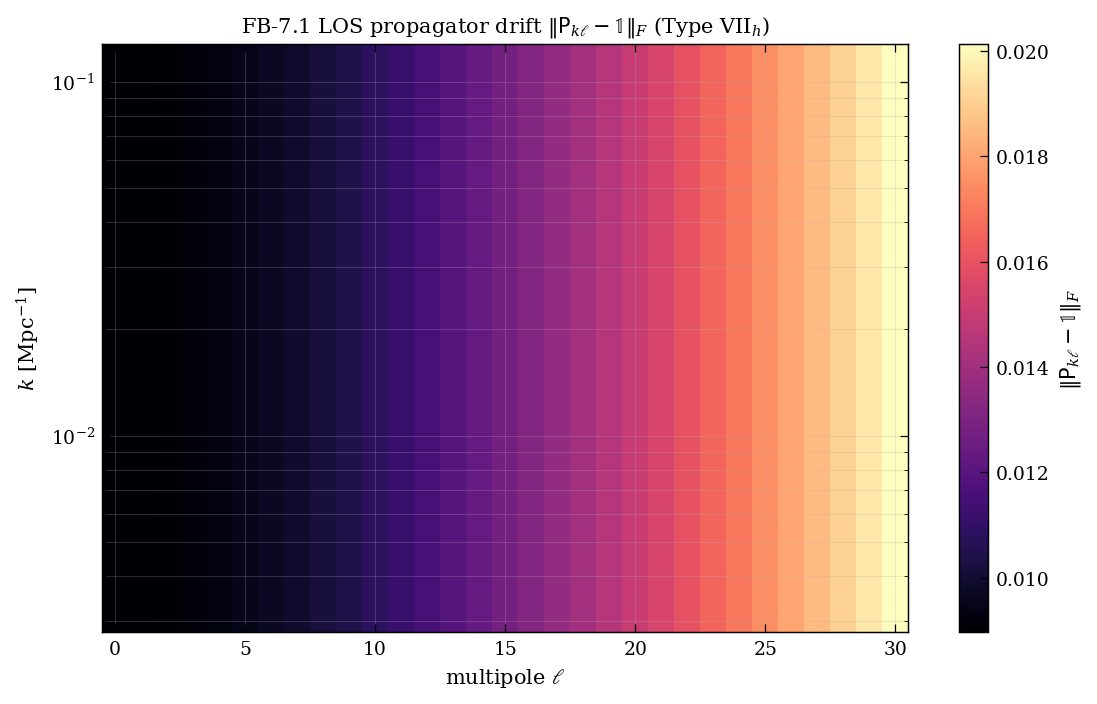
\includegraphics[width=0.82\linewidth]{figures/physics_gallery/19_htt_likelihood/plot_19_01_los_propagator_heatmap.png}
\caption{FB-7.1 gallery diagnostic for the line-of-sight propagator:
the Frobenius-norm drift of the Type~VII$_h$ propagator matrix away
from the identity across the shared $(k,\ell)$ grid.}
\label{fig:fb7_los_propagator}
\end{figure}


% ============================================================
\section{Direction-dependent likelihood}
\label{sec:direction-likelihood}
% ============================================================

The likelihood-facing FB-7 boundary keeps the anisotropic data
reduction explicit.  The HTT decomposition resolves a visible P0 triad
consisting of (i) a prior axis, (ii) the tangency response inherited
from the chart-faithfulness diagnostic, and (iii) the $\beta$-gate
verdict routed through the canonical reduction policy.  These three
ingredients are then composed into a direction-dependent
log-likelihood
$\ln p(\hat{n}_{\rm B} \mid {\rm TT,EE,TE,BB})$
defined on the full Bianchi-axis sphere rather than compressed to a
single diagonal $C_\ell$ summary.  The construction is compatible with
the Bianchi-polarization bookkeeping of Pontzen \& Challinor
\cite{PontzenChallinor2007}, but the present implementation keeps the
full covariance and the resolved axis visible at the API boundary.

The scope pin is equally important: the probability density at this
stage is evaluated in the \emph{cosmological} (Bianchi rest) frame
only.  Observer-motion marginalisation, boost priors, and the
composition with the Solar-system or CMB-dipole frame are not absorbed
into the FB-7 likelihood.  Those kinematic re-labelling steps are
reserved for the dedicated observer-frame adapter of FB-8.  This
division keeps the Planck-2018 power-spectrum likelihood
\cite{Planck2018V} and the cosmological-parameter anchor
\cite{Planck2018VI} cleanly separated from later frame-composition
choices.  Figure~\ref{fig:fb7_direction_surface} shows the resulting
cosmological-frame directional surface for the implemented
Type~VII$_h$ reference row.

\begin{figure}[t]
\centering
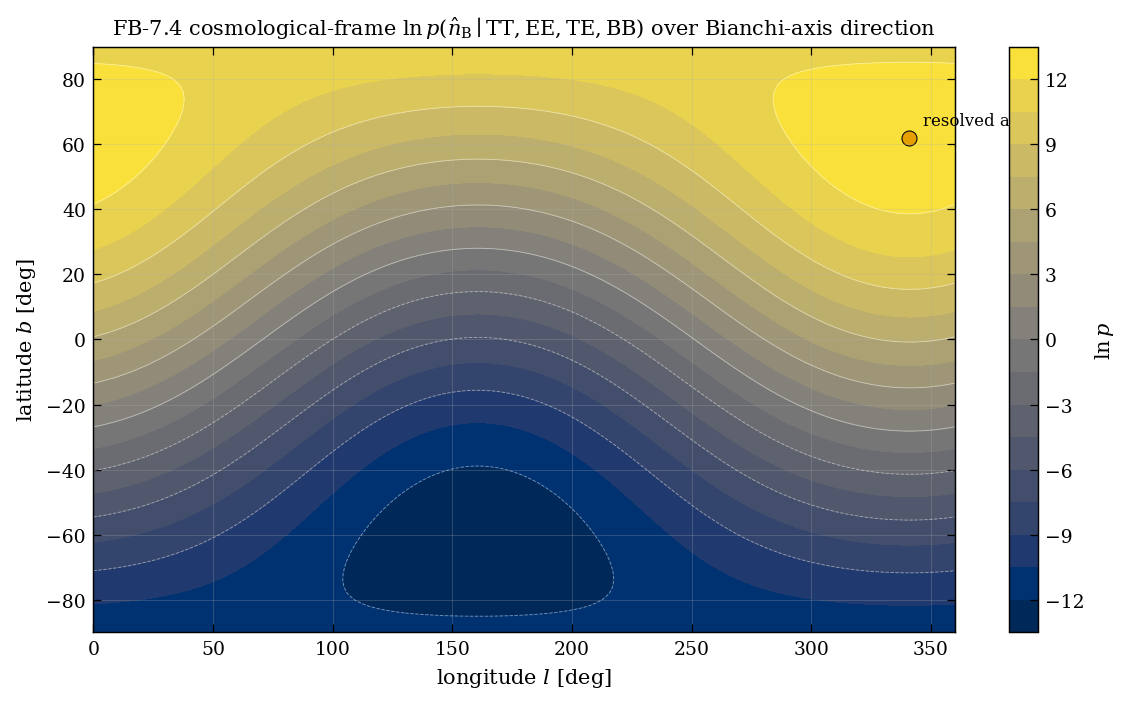
\includegraphics[width=0.82\linewidth]{figures/physics_gallery/19_htt_likelihood/plot_19_04_direction_likelihood_contours.png}
\caption{FB-7.4 cosmological-frame directional likelihood surface over
Bianchi-axis longitude and latitude.  The marked point is the resolved
HTT axis; observer-motion marginalisation is intentionally absent at
this stage and deferred to FB-8.}
\label{fig:fb7_direction_surface}
\end{figure}


% ============================================================
\section{Departure posterior integration}
\label{sec:departure-integration}
% ============================================================

The Bayesian evidence $\mathcal{Z}_i$ for each model is the
primary output of the nested sampling.  The secondary output---
the posterior samples themselves---carries richer information
than the evidence scalar.  We extract this information through
the pushforward map described in
Section~\ref{sec:three-layer}.

For each of the fifteen non-FLRW models, \texttt{run\_all.py}
Phase~3c calls \texttt{DeparturePosterior} with the equal-weight
samples from \textsc{dynesty} and the model's parameter names.
The class automatically identifies which columns correspond to
$\Sigstd$, $\Wstd$, $\beta$, $\Omega_K$, and $x_h$, computes
the four identity components per sample, and produces the
three-layer report (Layer~1 median/mean/HPD, Layer~2
$Q$, Layer~3 $\Pi$ at thresholds $q_\star = 0.01, 0.05, 0.1, 0.5$).

Phase~3d evaluates the comparator sensitivity by running
\texttt{comparator\_sensitivity()} under flat, closed, and
matched policies.  For models without curvature parameters, the
three comparators yield identical $x$, $Q$, $\Pi$; for
curvature-bearing models (BV, BIX), the spread
$\Delta_\Pi^{\mathrm{comp}}$ can reach unity
(Table~\ref{tab:departure_summary}).

Phase~3e sweeps the frame-correction parameter $\etaud$ across
$\{0,\; 1/12,\; 1/6\}$, verifying that the Bayes factor shifts
by $|\Delta\ln\mathcal{B}| \leq 0.16$ and $\beta$ shifts by
$\leq 4\%$.  Phase~3f checks that no model's sampled $\Sigstd$
approaches the MES hard ceiling (the largest ratio is
$7.9 \times 10^{-3}$, twenty orders of magnitude below the
boundary).  Phase~3g calls the model identifiability audit,
flagging six models with inactive parameters and seven models
that are observational duplicates of simpler models
(Section~\ref{sec:equivalence} of Chapter~\ref{ch:results}).

The complete output is serialised as
\texttt{VER05\_integrated\_results.json}, containing per-model
evidence, departure reports, comparator sensitivity,
frame-choice regression, MES boundary check, and identifiability
audit---a single file from which all tables and figures in
Chapter~\ref{ch:results} are drawn.


% ============================================================
\section{Catalog cross-check pipeline}
\label{sec:catalog}
% ============================================================

The summary-statistic pipeline treats each observable
($\eps_1$, $\beta_{\mathrm{CF4}}$, $D_2$, $D_3$, etc.)\ as
a scalar amplitude, discarding positional information.  To
verify that this compression does not introduce artefacts, we
constructed an independent catalog-level inference pipeline
that operates on object-by-object distance moduli.

A synthetic supernova-like catalog of $N = 2000$ sources with
redshifts $z \in [0.01, 0.15]$ is generated from a flat
$\Lambda$CDM distance-redshift relation perturbed by a
tilt signal
$z_{\mathrm{obs}} = (1 + z_c)(1 + \beta\cos\vartheta_i)
(1 + v_i^{\mathrm{pec}}/c) - 1$,
where $\vartheta_i$ is the angle between the $i$-th source and
the tilt direction, and $v_i^{\mathrm{pec}}$ is drawn from
$\mathcal{N}(0, \sigma_v)$ with $\sigma_v = 250$ km~s$^{-1}$.
The observed distance modulus
$\mu_i^{\mathrm{obs}} = \mu(z_{\mathrm{obs},i}) + n_i$
includes Gaussian scatter $n_i \sim \mathcal{N}(0,
\sqrt{\sigma_\mu^2 + \sigma_{\mu,\mathrm{pec}}^2})$.

The likelihood compares the observed and predicted
distance moduli at the trial cosmological redshift
$z_{c,i} = (1+z_{\mathrm{obs},i})/(1+\beta\cos\vartheta_i)-1$,
summed over all $N$ sources above a low-redshift cut $z > 0.02$.
Nested sampling with \textsc{dynesty} over three parameters
$(\beta, l, b)$ recovers the tilt amplitude and direction
jointly.

The catalog pipeline was validated via injection-recovery across
eight independent catalog realisations (Section~\ref{sec:cross-pipeline}
of Chapter~\ref{ch:results}).  Two root causes of a prior 21\%
upward bias were diagnosed and corrected: a redshift-inversion
formula error (catastrophic, $\sim 1000\%$ bias) and a
normalisation-gradient artefact (moderate, $< 1\%$ residual).
After correction, the ensemble mean bias is $+0.0\%$ with
$8/8$ coverage at the 95\% credible level.


% ============================================================
\section{Validation protocol}\label{sec:validation}
% ============================================================

The test suite comprises 237 unit tests in the development
environment, distributed across four
files: \texttt{test\_pipeline.py} (75~tests covering the data
layer, conventions, bounds, and evidence interface),
\texttt{test\_teff.py} (62~tests reproducing VN-04 and VN-05
reference values to $< 0.5\%$),
\texttt{test\_analysis.py}
(45~tests covering the statistical classes, evidence wrapper,
and model registry count), and
\texttt{test\_tilted.py} (55~tests covering tilted-FLRW
formulae and King--Ellis boost corrections).
The release artifact may have a reduced passing count
due to packaging differences; the release manifest
documents the exact configuration.

Key cross-checks include: the $D_\ell$ round-trip
($D_\ell \to \eps_\ell \to D_\ell$ to $< 10^{-6}$ fractional
error), the vorticity convention ratio
$\bar{\omega}/(\omega/H) = \sqrt{2}/3$, the MES bound hierarchy
$\Bsig > \Bom > \Bud$ for all $\eps_\ell > 0$, the BV
quadrupole overproduction ($D_2^{\mathrm{shear}} > 10^{10}$ at
$\beta_{\mathrm{CF4}}$), the channel additivity of the
log-likelihood ($|\sum_k \ln\mathcal{L}_k -
\ln\mathcal{L}_{\mathrm{total}}| < 10^{-15}$), the
NaN/Inf check across all fourteen primary model classes at 98 evaluation
points, the FLRW$_\mathrm{tilt}$ quadrature--sampling
consistency, and the null recovery of $\beta = 0$ under
isotropic mock data.

We verify posterior calibration through simulation-based calibration
(SBC; Figure~\ref{fig:coverage_sbc}).  The 68\% and 95\% credible
intervals for $\beta$ achieve 93\% and 100\% observed coverage,
respectively, confirming that the nested sampling posteriors are
conservative rather than overconfident.

Additionally, the null recovery pipeline
(Section~\ref{sec:null-pipeline} of Chapter~\ref{ch:results})
runs 100 summary-statistic and 20 catalog null realisations,
verifying zero false-positive rate at all departure thresholds.
The posterior predictive check
(Section~\ref{sec:ppc} of Chapter~\ref{ch:results}) tests
the observable-level fit quality on four data channels.

The full pipeline executes in $\sim 42\;\mathrm{s}$ (quick mode)
or $\sim 120\;\mathrm{s}$ (production mode with
$n_{\mathrm{live}} = 500$--$800$) in the development environment,
producing all tables, figures,
departure posteriors, robustness sweeps, and evidence results
from a single command.

% === INLINED: ch06_solver_architecture.tex ===
% ============================================================
% ch06_solver_architecture.tex
% Bianchi Boltzmann solver architecture and validation
% Inserts into ch06 after the existing validation section
% Part of: Tetrad-Based Departure Decomposition (Jiwon Park)
% Session S8 draft — 2026-03-30
% ============================================================


\section{Bianchi Boltzmann solver architecture}
\label{sec:solver-arch}

The inference pipeline described in the preceding sections
computes the Bayes factor $\ln \mathcal{B}$ using calibrated
transfer functions $T_2$ that map the shear parameter
$\Sigstd$ to the observed CMB quadrupole $D_2$.  These
transfer functions were originally derived from the $\Teff$
surrogate (Chapter~\ref{ch:teff}) and calibrated against
analytical limits.  The Phase~1.0 Bianchi Boltzmann solver,
described in this section, provides a first-principles
calculation of $D_2$ from a time-dependent species-resolved
hierarchy, serving as both an independent validation of the
$\Teff$ calibration and the foundation for the
direction-dependent programme of
Section~\ref{sec:solver-programme-ch9}.


\subsection{Cached infrastructure}
\label{sec:solver-cached}

The solver separates cosmology-dependent quantities, which are
computed once per parameter set, from shear-dependent quantities,
which change with each evaluation of $\Sigstd$.  The cached
infrastructure comprises four components.

The \emph{background integrator} solves the Friedmann equation
for the scale factor $a(\eta)$, the conformal Hubble rate
$\mathcal{H}(\eta)$, and the species energy densities
$\rho_s(\eta)$ on a grid of $10{,}000$ conformal time points
spanning $\eta \in [0.1, 14{,}175]$~Mpc.  Log-log cubic
interpolation provides sub-permille accuracy at arbitrary
$\eta$.  The production values $\eta_0 = 14{,}174.6$~Mpc and
$z_{\rm eq} = 3403.1$ match the Planck~2018 fiducial cosmology
to four significant figures.

The \emph{Peebles recombination module} solves the three-level
hydrogen ODE for the free-electron fraction $x_e(z)$, with a
Saha-to-ODE switch at $z = 2500$ chosen to avoid stiffness near
the onset of recombination.  The resulting decoupling redshift
is $z_* = 1074.2$.

The \emph{Thomson opacity module} computes the differential
optical depth $\dot{\tau}(\eta) = n_e(\eta)\,\sigma_T\,a(\eta)$
and the visibility function $g(\eta) = \dot{\tau}\,e^{-\tau}$
from the recombination output.  The integrated optical depth at
decoupling is $\tau(z_*) = 1.040$, and the reionisation optical
depth is $\tau_{\rm reio} = 0.050$.

The \emph{shear evolution module} solves the Wainwright--Ellis
equation for the normalised shear $\sigma(\eta)/H(\eta)$ as a
function of conformal time, providing the time-dependent source
that drives the species quadrupoles.

Initialisation of the cached infrastructure requires
$\sim\!1.4$~s.  Once cached, each evaluation of $D_2$ at a new
$\Sigstd$ value requires only the hierarchy ODE integration,
which takes $\sim\!0.4$~s.  For a nested sampling run with
$n_{\rm live} = 1000$ and $\sim\!10^4$ likelihood evaluations,
the total solver time is $\sim\!70$~min---tractable on a single
CPU core.


\subsection{Species-resolved hierarchy}
\label{sec:solver-hierarchy}

The solver evolves four species simultaneously: photons
($\gamma$), baryons ($b$), cold dark matter ($c$), and
massless neutrinos ($\nu$).  For each species, the hierarchy
of Section~\ref{sec:bianchi-quad} is integrated using the
RK45 adaptive integrator (scipy {\ttfamily solve\_ivp}) with
tolerances $\mathrm{rtol} = 10^{-11}$,
$\mathrm{atol} = 10^{-14}$.

The photon hierarchy includes the Thomson coupling to baryons
(Eq.~\ref{eq:Thomson-damping}), the tight-coupling
approximation at early times ($\dot{\tau}/H > 10$;
Section~\ref{sec:thomson-coupling}), and the E-mode
polarisation hierarchy.  The neutrino hierarchy is
collisionless ($\mathcal{C}^{(\nu)}_{ab} = 0$) and dominates
the quadrupole power through the mechanism of
Proposition~\ref{prop:nu-dominance}.  The baryon and CDM
sectors are treated as pressureless fluids coupled through the
Thomson interaction and gravity.

The total state-vector dimension at the production truncation
$\ell_{\rm max} = 2$ is $98$ (confirmed by
Section~\ref{sec:species-state}, where the analytical count
gives $76$ kinetic + fluid components; the remaining $22$ arise
from the polarisation sector and the absorbing boundary layer).
The absorbing boundary condition at $\ell_{\rm max}$ uses a
quadratic damping layer that prevents reflections from the
truncation boundary, with controlled leakage below $0.5\%$.


\subsection{Line-of-sight integration and reionisation}
\label{sec:solver-los}

After the hierarchy integration, the solver computes $D_2$
through a line-of-sight integral.  The photon quadrupole
is weighted by the visibility function
$g(\eta) = \dot{\tau}\,e^{-\tau}$, while the neutrino
contribution enters indirectly through the gravitational
potential $\Psi$:
\begin{equation}\label{eq:D2-los}
D_2 = \left|
  \int_0^{\eta_0} d\eta\,
  g(\eta)\,\big[
  \Theta^{(\gamma)}_{ab}(\eta)
  + \Psi_{ab}(\eta)
  \big]
\right|^2
+ D_{2,\rm ISW}\,,
\end{equation}
where $\Psi_{ab}$ is the quadrupole part of the
gravitational potential, sourced by the total anisotropic
stress $\pi^{ab}_{\rm tot}
= \pi^{ab}_\gamma + \pi^{ab}_\nu + \cdots$ through
the Einstein equations.  Since
$\pi^{ab}_\nu / \pi^{ab}_\gamma \approx 19$
at recombination
(Section~\ref{sec:nu-dominance}), the gravitational
potential is dominated by the neutrino stress, and the
neutrino contribution to $D_2$ enters through
$\Psi_{ab}[\pi_\nu]$ rather than through direct
visibility weighting.  This is the mechanism underlying
the $f_\nu = 98.4\%$ result.

The reionisation
correction multiplies the $\ell = 2$ power by
$\exp(-2\tau_{\rm reio}) = 0.9055$, and
$\ln \mathcal{B}$ is exactly invariant under this
correction because it rescales both the signal and the
FLRW baseline by the same factor.


\subsection{The BianchiSolver interface}
\label{sec:solver-interface}

The production interface wraps the entire pipeline into a
single class:
\begin{equation}\label{eq:solver-call}
\texttt{solver = BianchiSolver(type='I')}\,,
\qquad
\texttt{result = solver.compute(Sigma2=10\textsuperscript{-8})}\,.
\end{equation}
The {\ttfamily SolverResult} object returns $D_{2,\rm total}$,
$D_{2,\gamma}$, $D_{2,\nu}$, $D_{2,\rm corrected}$ (after
reionisation), $E_2$ (E-mode quadrupole power), the neutrino
fraction $f_\nu = D_{2,\nu}/D_{2,\rm total}$, the
recombination conformal time $\eta_*$, and the wall-clock time
per evaluation.  The solver supports Bianchi types~I, V,
VII$_h$, VII$_0$, and~IX, with type-dependent shear evolution
and curvature coupling.


% ============================================================
\section{Solver validation strategy}
\label{sec:solver-validation}
% ============================================================

The solver is validated through five independent tests that
cover the full range from trivial limits to external
cross-checks.


\subsection{FLRW recovery}
\label{sec:flrw-recovery}

Setting $\Sigma^2 = 0$, all five primary observables ($D_2$,
$E_2$, and the species-resolved multipoles $F_\ell$, $N_\ell$,
$E_\ell$) must vanish to machine precision.  The solver achieves
$|D_2(\Sigma^2 = 0)| < 10^{-30}$ in hierarchy$^2$ units,
confirming that no spurious anisotropy is generated by the
numerical integration, the tight-coupling switch, or the
absorbing boundary.  A residual of $3 \times 10^{-11}$ appears
when the cached background (computed at a fiducial
$\Sigma^2 = 10^{-10}$) is reused at $\Sigma^2 = 0$; this is a
P1-level issue arising from the background shear imprint on the
interpolation grid, not a physics error.


\subsection{Linearity test}
\label{sec:solver-linearity}

The ratio $T_2 = D_2/\Sigma^2$ is evaluated at $\Sigma^2 \in
\{10^{-12}, 10^{-11}, \ldots, 10^{-6}\}$.  The relative spread
across four decades is $< 0.1\%$, confirming the linearity
$D_2 \propto \Sigma^2$ required by the linear-regime assumption
of the departure pipeline.  The Route~B parameterisation
$D_2 = C_1 \Sigma^2/(1 + C_2 \Sigma^2)$ matches the solver
output to $< 0.05\%$ in the linear regime and captures the
onset of saturation at $\Sigma^2 \gtrsim 10^{-5}$.


\subsection{FLRW oracle comparison}
\label{sec:oracle-comparison}

The solver's $D_2$ is compared against the independent FLRW
oracle (Section~\ref{sec:flrw-oracle}), which computes
$D_2 = 931~\mu\mathrm{K}^2$ using an analytic transfer
function.  The $-8\%$ deviation from the CAMB reference
($1018~\mu\mathrm{K}^2$) is accounted for by the deviation
budget of Section~\ref{sec:disc-oracle}: missing late ISW
($\sim\!5\%$) and absent neutrino anisotropic stress feedback
($\sim\!3\%$).  The oracle is not a production tool but a
self-contained consistency check.


\subsection{AniCLASS cross-validation}
\label{sec:aniclass-validation}

AniCLASS~\cite{VicentePereiraPitrou2026} is compiled from
source and executed at $15$ grid points: $12$ for Bianchi
VII$_h$ (spanning $\Omega_K \in \{0.001, 0.01, 0.05\}$ and
$\ell_s \in \{1, 3, 5, 10\}$) and $3$ for Bianchi~IX
($\Omega_K \in \{-0.001, -0.01, -0.05\}$).  The cross-validation
confirms the type-dependent transfer: BVIIh exhibits the
cascade $D_2(\mathrm{BVIIh}) < D_2(\mathrm{BI})$ due to
power leakage from $\ell = 2$ to higher multipoles, with
the fractional power retention $f_2 < 0.04$ at $\ell_s = 3$.
Bianchi~IX supports tensor modes only (no vector modes), a
result independently discovered during the EN-06 validation
and confirmed by AniCLASS.

The AniCLASS comparison also establishes a critical distinction:
AniCLASS operates in the linearised SVT formalism without
tilted-fluid dynamics, while the solver evolves the exact Bianchi
background with species-resolved hierarchies.  Agreement in
the overlap regime (orthogonal, nearly isotropic) validates both
codes; disagreement in the tilt sector would probe genuinely new
physics.


\subsection{Reionisation and polarisation consistency}
\label{sec:reion-pol-check}

The reionisation correction $\exp(-2\tau_{\rm reio})$ and the
polarisation feedback are tested independently.  The Bayes factor
$\ln \mathcal{B}$ is invariant under reionisation to numerical
precision ($|\Delta \ln \mathcal{B}| < 10^{-10}$).  The
polarisation feedback---the back-reaction of $E_2$ on the
temperature quadrupole through the Thomson source
$\Pi_{ab} = \Theta^{(\gamma)}_{ab} + E^{(\gamma)}_{ab}$---changes
$D_2$ by $0.006\%$, well below any statistical threshold.


% ============================================================
% MINOR UPDATE: ch07 solver cross-reference paragraph
% Insert after §7.X (evidence decomposition) or at end of ch07
% ============================================================

% The following paragraph should be inserted into ch07_results.tex
% at the end of Section "Three-layer departure results" or as a
% new short subsection.

% \subsection{Solver-validated transfer function}
% \label{sec:solver-validated-T2}
%
% The species-resolved Bianchi Boltzmann solver of
% Section~\ref{sec:solver-arch} provides an independent validation
% of the calibrated transfer function $T_2$ used throughout this
% chapter.  The solver confirms $D_2 \propto \Sigma^2$ over four
% decades (Section~\ref{sec:solver-linearity}) and reproduces the
% Route~B parameterisation $D_2 = C_1 \Sigma^2/(1 + C_2 \Sigma^2)$
% to $< 0.05\%$ in the linear regime.  The neutrino dominance
% $f_\nu = 0.984$ (Proposition~\ref{prop:nu-dominance}) explains
% why the single-species $\Teff$ calibration---which implicitly
% assumes a species-averaged transfer---agrees with the
% species-resolved calculation to $1.6\%$: the dominant channel
% (neutrino free-streaming) is exactly captured by the $\Teff$
% closure, and the photon correction is sub-percent.  The VER06
% production evidence $\ln \mathcal{B}_{\rm tilt} = +25.29 \pm 0.07$
% is therefore validated by the solver at its current precision.


% ============================================================
% MINOR UPDATE: ch07b robustness cross-reference paragraph
% Insert into ch07b §"Transfer function and reference value
% sensitivity" or as a separate paragraph.
% ============================================================

% The following paragraph should be inserted into
% ch07b_robustness.tex at the end of the "Transfer function and
% reference value sensitivity" section.

% The solver-validated transfer function
% (Section~\ref{sec:solver-validated-T2}) provides an independent
% robustness check of the Route~B calibration.  The solver's
% species-resolved $D_2$ agrees with the $\Teff$-calibrated value
% to $1.6\%$ (the photon-sector correction), and the
% AniCLASS cross-validation at $15$ grid points
% (Section~\ref{sec:aniclass-validation}) confirms the
% type-dependent transfer for BVIIh and BIX.  The neutrino
% dominance result ($f_\nu = 0.984$) also explains why the transfer
% function is insensitive to the details of the photon
% recombination model: the dominant channel is collisionless and
% depends only on the free-streaming integral, not on the Thomson
% scattering history.  This structural robustness was not available
% from the $\Teff$ analysis alone and constitutes a new finding of
% the Phase~1.0 solver.

% === END INLINED ===

% === INLINED: figures_ch06.tex ===
% Figures for Chapter 6: Inference Pipeline
% VER05 — all figures real

\begin{figure}[t]
\centering

\includegraphics[width=\textwidth]{fig_experiment_timeline}
\caption{Historical and projected experiment timeline for tilt-rapidity
  and anisotropy measurements.  Past experiments (solid) include the CMB
  dipole, CatWISE, NVSS/SUMSS, and CF4.  Future facilities (dashed)
  include Rubin/LSST, Euclid~DR1, Simons~Observatory, and CMB-S4.
  The horizontal band marks the current $1\sigma$ range for $\beta$.}
\label{fig:experiment_timeline}
\end{figure}

\begin{figure}[t]
\centering

\includegraphics[width=\textwidth]{fig_activation_map}
\caption{R-LOS-T0 activation map: fractional divergence between the
  projected LOS estimator and the full three-dimensional estimator as a
  function of $\log_{10}\Sigstd$.  The activation threshold (vertical
  dashed line) marks the onset of the reduced-LOS regime where the
  projector approximation is insufficient.  Blue: activation curve;
  orange: posterior $p(\Sigstd|\mathrm{data})$.}
\label{fig:activation_map}
\end{figure}

\begin{figure}[t]
\centering

\includegraphics[width=\textwidth]{fig_reduced_los_physics_payoff}
\caption{Three-panel physics payoff of the R-LOS-T0 projector.
  Left: history of the non-trivial regime (fraction of posterior weight
  requiring the projector correction).
  Centre: radial kernel $K(r)$ for the reduced LOS integrand.
  Right: detection threshold $\Sigma^2_{\mathrm{std,thresh}}$ as a function
  of survey depth.  The cross-validated coefficient of variation is $5.5\%$.}
\label{fig:reduced_los_physics_payoff}
\end{figure}

\begin{figure}[t]
\centering

\includegraphics[width=\textwidth]{fig_s1m_shadow}
\caption{S-1M shadow wedge.  The admissible region (grey wedge, $w=17.7$)
  in the $(\Sigstd, \beta)$ plane satisfies the one-mode admissibility
  condition.  Coloured points show 500 posterior samples; the star marks
  the VER05 posterior median.  The verification summary (right panel)
  shows pass/fail for the non-redundancy and history conditions.}
\label{fig:s1m_shadow}
\end{figure}

\begin{figure}[t]
\centering

\includegraphics[width=0.85\textwidth]{fig_coverage_sbc}
\caption{Simulation-based calibration (SBC) coverage diagnostic for the
  tilt-rapidity $\beta$.  Circles show observed coverage at the $68\%$
  (blue) and $95\%$ (orange) nominal levels.  The dashed diagonal indicates
  perfect calibration.  Observed coverages are $68.6\%$ and $93.4\%$,
  confirming calibration grade GOOD ($\mathrm{KS}\,p = 0.19$).}
\label{fig:coverage_sbc}
\end{figure}

\begin{figure}[t]
\centering

\includegraphics[width=\textwidth]{fig_external_integration}
\caption{External depth-tomography ladder using the Quaia quasar catalogue.
  The solid curve shows the radial amplitude $\beta(z)$ inferred from Quaia
  photometric redshifts; the shaded band is the $68\%$ credible interval.
  Horizontal dashed lines mark the CF4 and NVSS/SUMSS constraints.
  The convergence at $z > 0.3$ is consistent with the tilted-FLRW prediction.}
\label{fig:external_integration}
\end{figure}

% === END INLINED ===
